% !TEX root = ../../vzor.tex
%% Ukázka: obrázky: wrapfigure, figure, subfigure; krátký název sekce
%% Vkládá ji soubor vzor/kapitoly/teorie.tex; ve vzor.pdf je pod nadpisem uvedeno „Zdroj ukázky".

\section[Obrázky]{Obrázky (ukázka krátkého názvu sekce v obsahu)}
%%% v obsahu se zobrazí jen text v hranatých závorkách – hodí se pro dlouhé nadpisy
\zdrojukazky{vzor/ukazky/obrazky.tex}

Obrázek s obtékáním textu – balíček \texttt{wrapfig} (obrázek~\ref{fig:wrap}):
\begin{wrapfigure}{r}{0.4\linewidth}
	\centering
	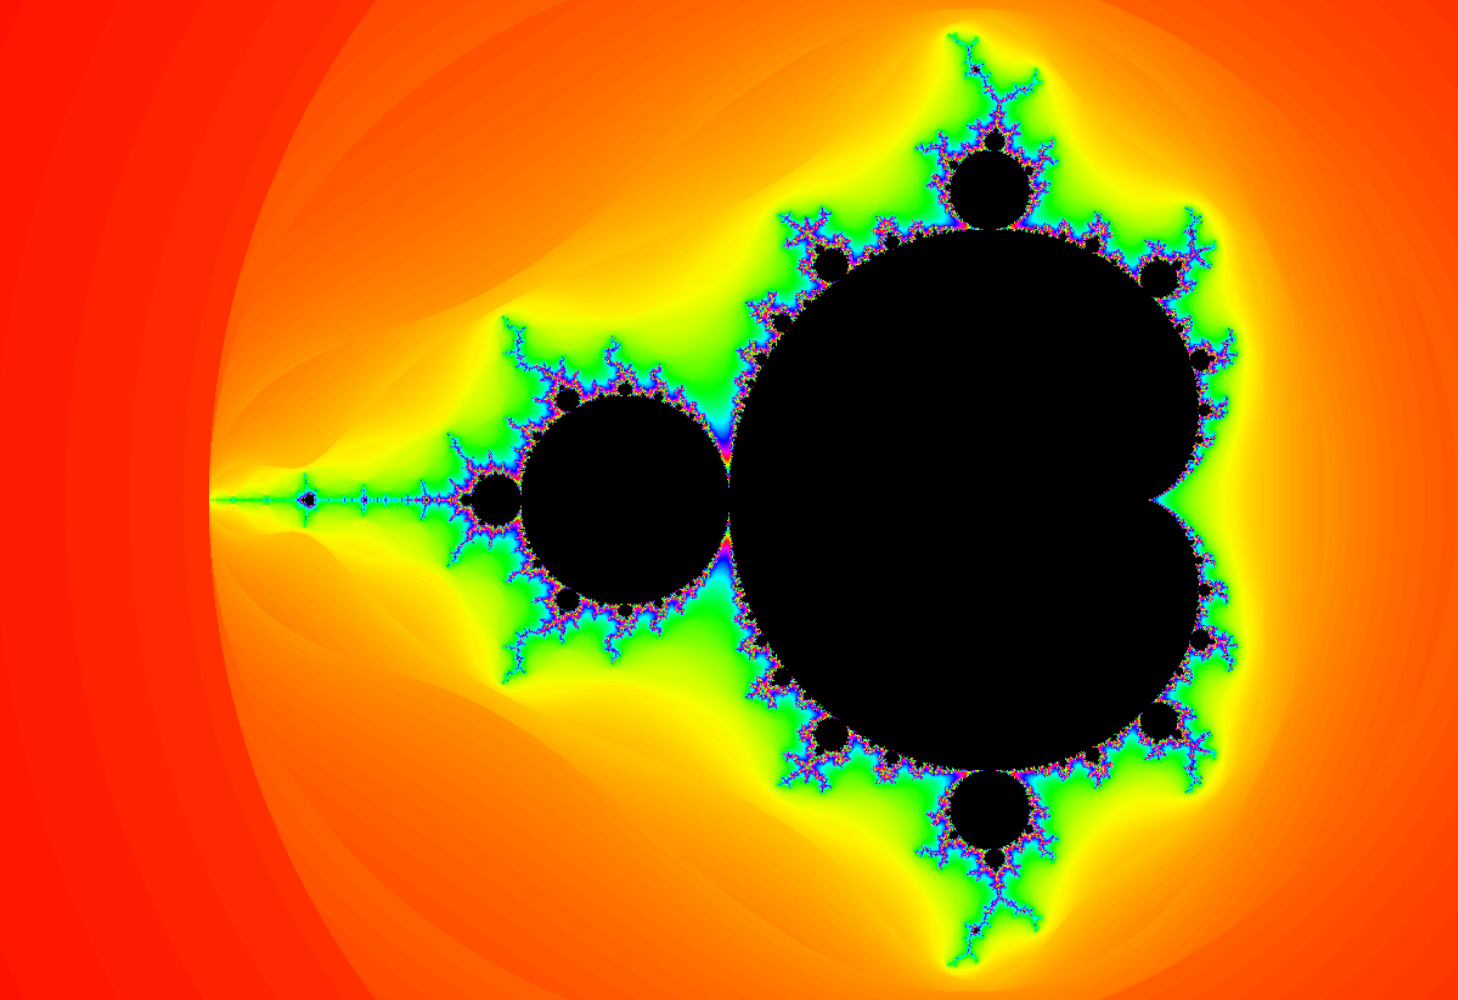
\includegraphics[width=\linewidth]{mandelbrot}
	\caption{Mandelbrotova množina}
	\label{fig:wrap}
\end{wrapfigure}
\lipsum[5]

Standardní obrázek přes celou šíři textu (obrázek~\ref{fig:test}):
\begin{figure}[htbp]
	\centering
	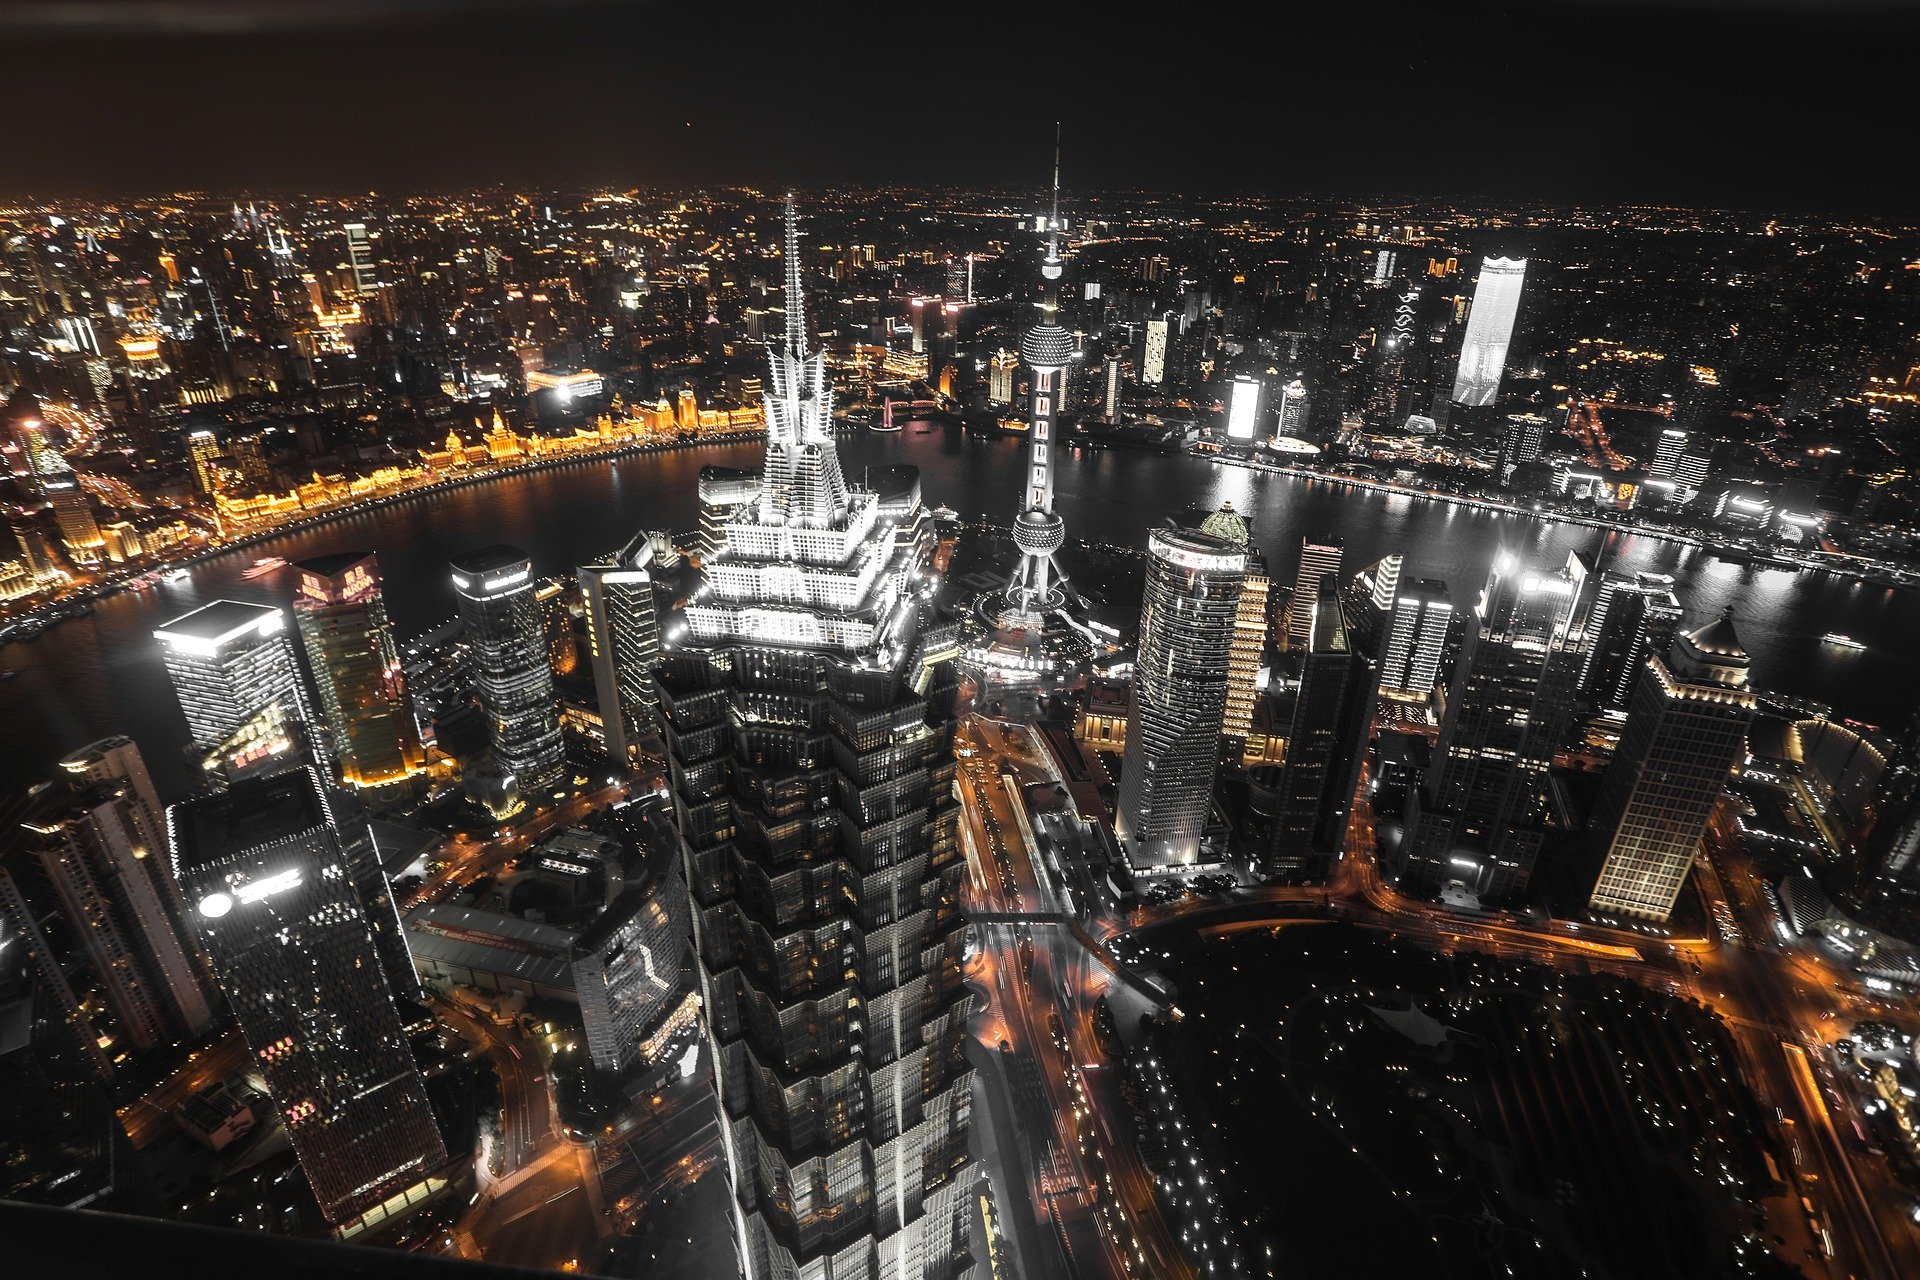
\includegraphics[width=\linewidth]{test.jpg}
	\caption{Šanghaj, zdroj: Pixabay}
	\label{fig:test}
\end{figure}

Tabulka~\ref{tab:mereni} obsahuje naměřené hodnoty.

\lipsum[3-5]

Dva obrázky vedle sebe – balíček \texttt{subcaption} (obrázky~\ref{fig:sub1} a~\ref{fig:sub2}):
\begin{figure}[htbp]
	\centering
	\begin{subfigure}{0.48\linewidth}
		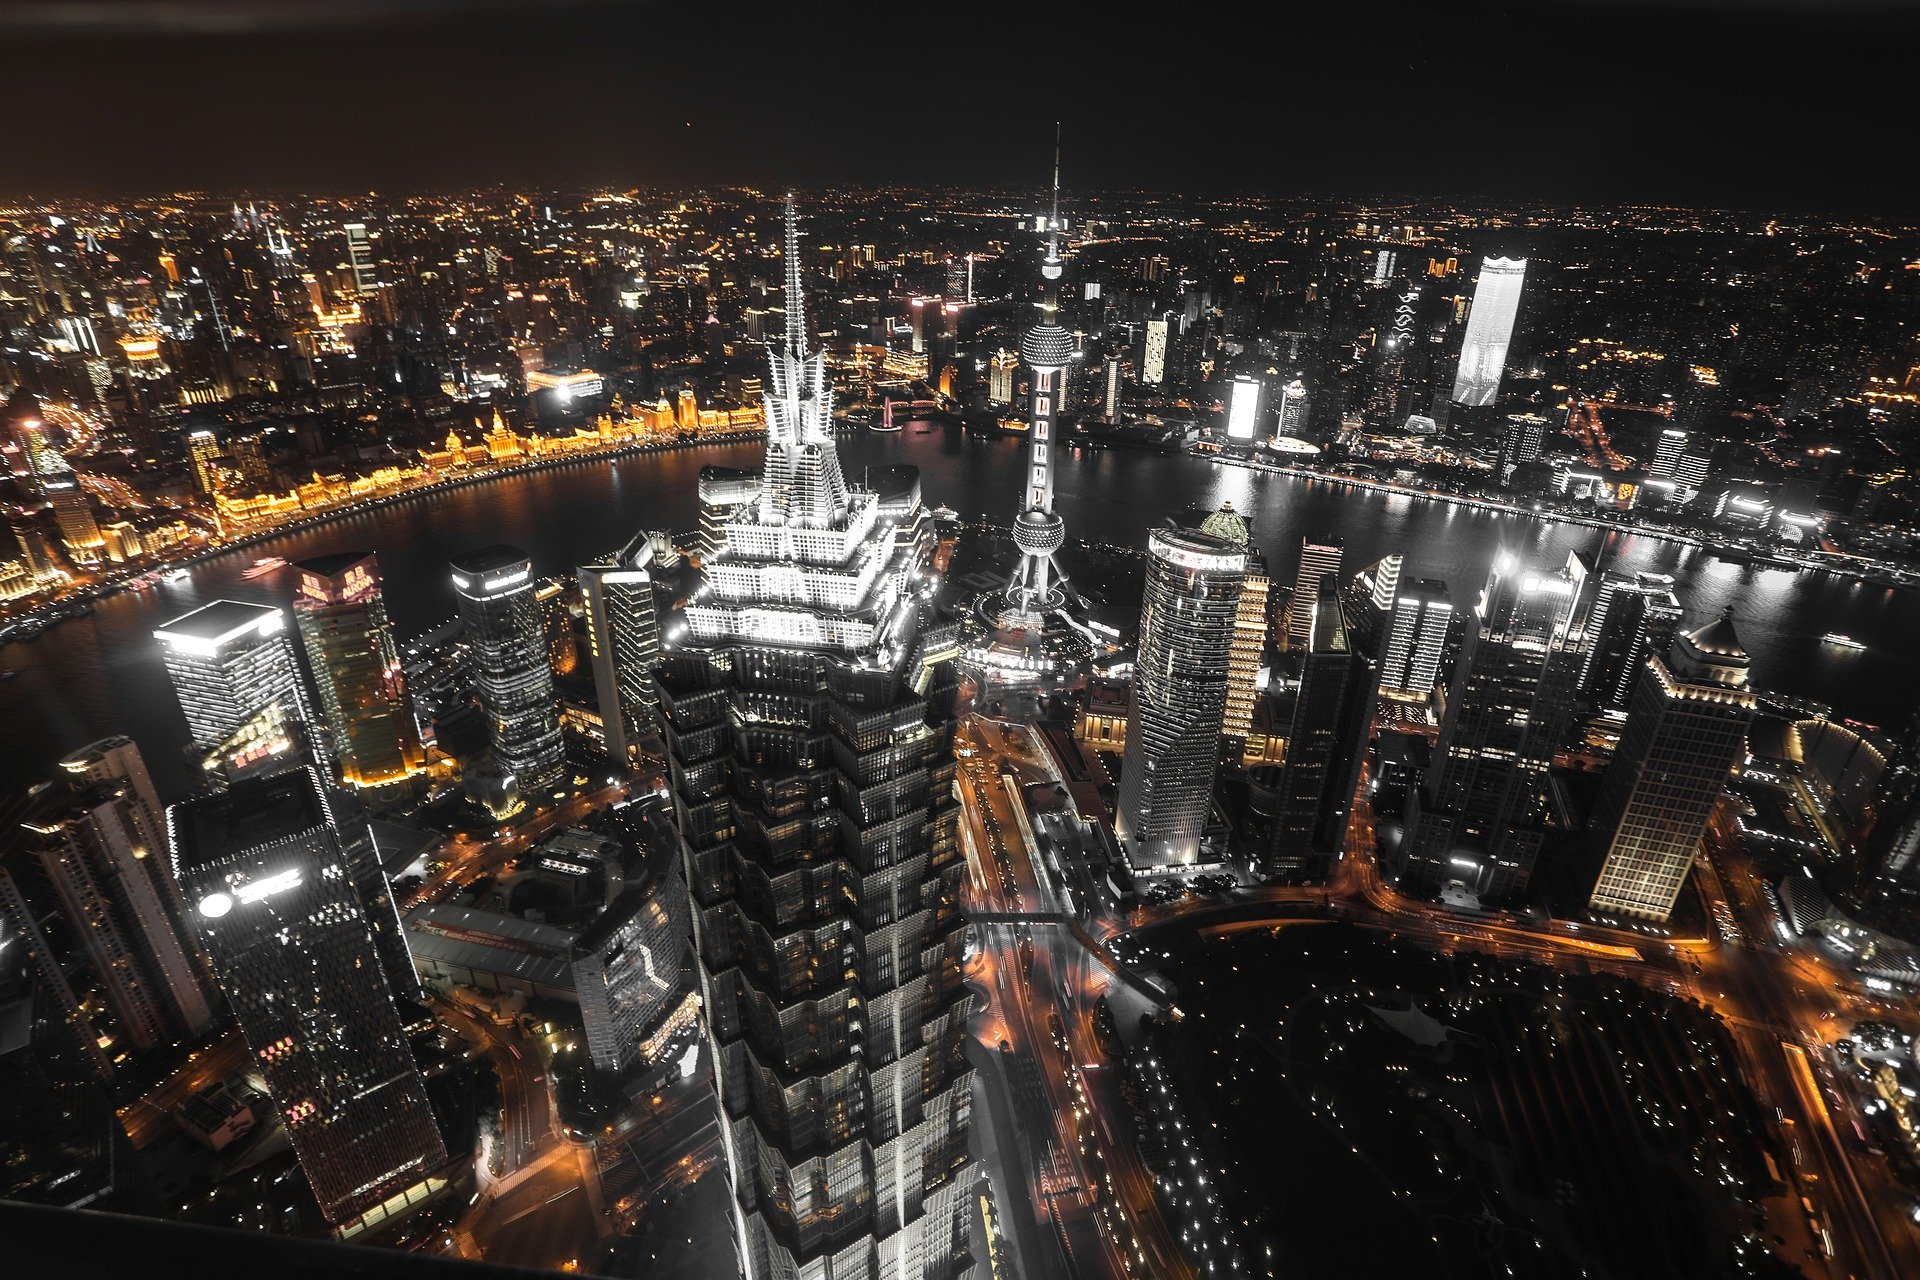
\includegraphics[width=\linewidth]{test.jpg}
		\caption{Šanghaj (Pixabay)}
		\label{fig:sub1}
	\end{subfigure}
	\hfill
	\begin{subfigure}{0.48\linewidth}
		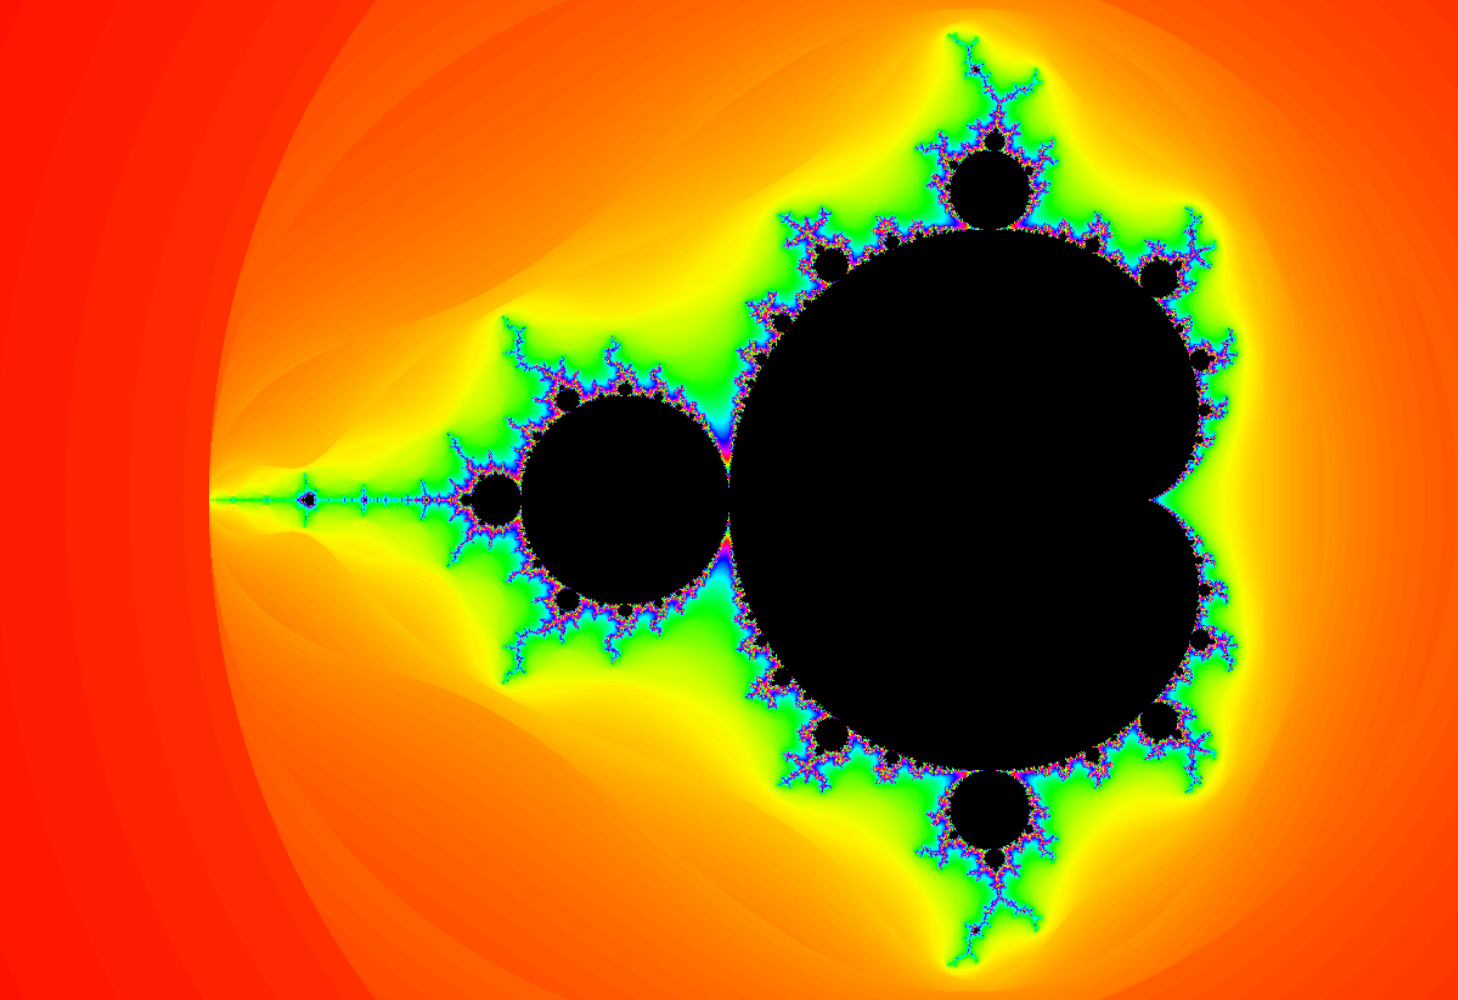
\includegraphics[width=\linewidth]{mandelbrot}
		\caption{Mandelbrotova množina}
		\label{fig:sub2}
	\end{subfigure}
	\caption{Dva obrázky vedle sebe}
	\label{fig:subfig}
\end{figure}

\lipsum[6]
